\startappendix{Dependence of Sensitivity on Signal Strength}
\label{chapter:appendix_mu_sig}

To assess the impact of varying the production rate of the DH signal model on the sensitivity of the search, Figure \ref{fig:limits_vary_mu_sig} compares the range of \ms and \mZp excluded by the search with the value of the signal strength parameter \(\mu\), which coherently scales the production rate of the DH signal process at all \ms and \mZp considered in the search. 

\begin{figure}[h]
  \centering
  \begin{subfigure}{0.48\textwidth}
    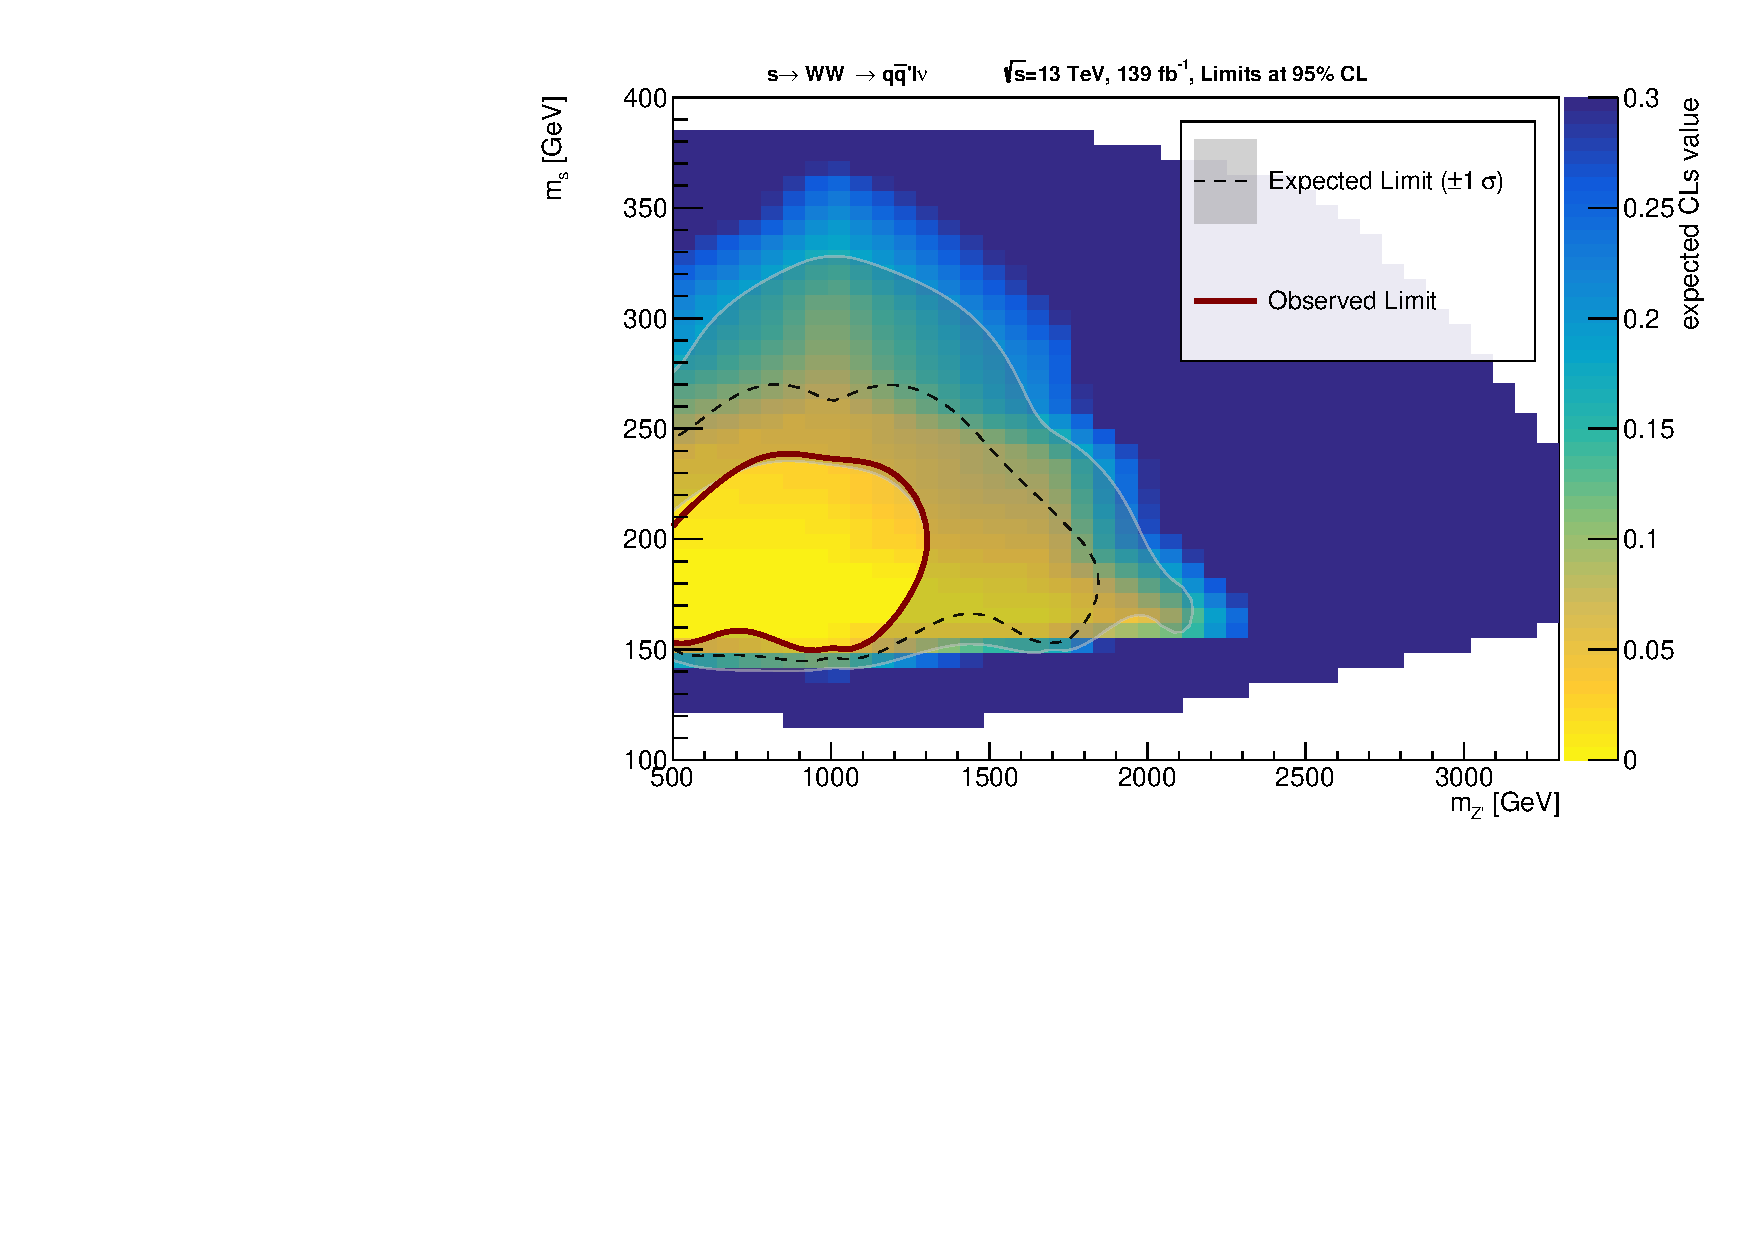
\includegraphics[width=\textwidth]{Figures/8/unblinded_0_20_nosig.pdf}
    \caption{\(g_q=0.20\)}\label{fig:unblinded_0.20}
  \end{subfigure} \hspace{0.3em}
  \begin{subfigure}{0.48\textwidth}
    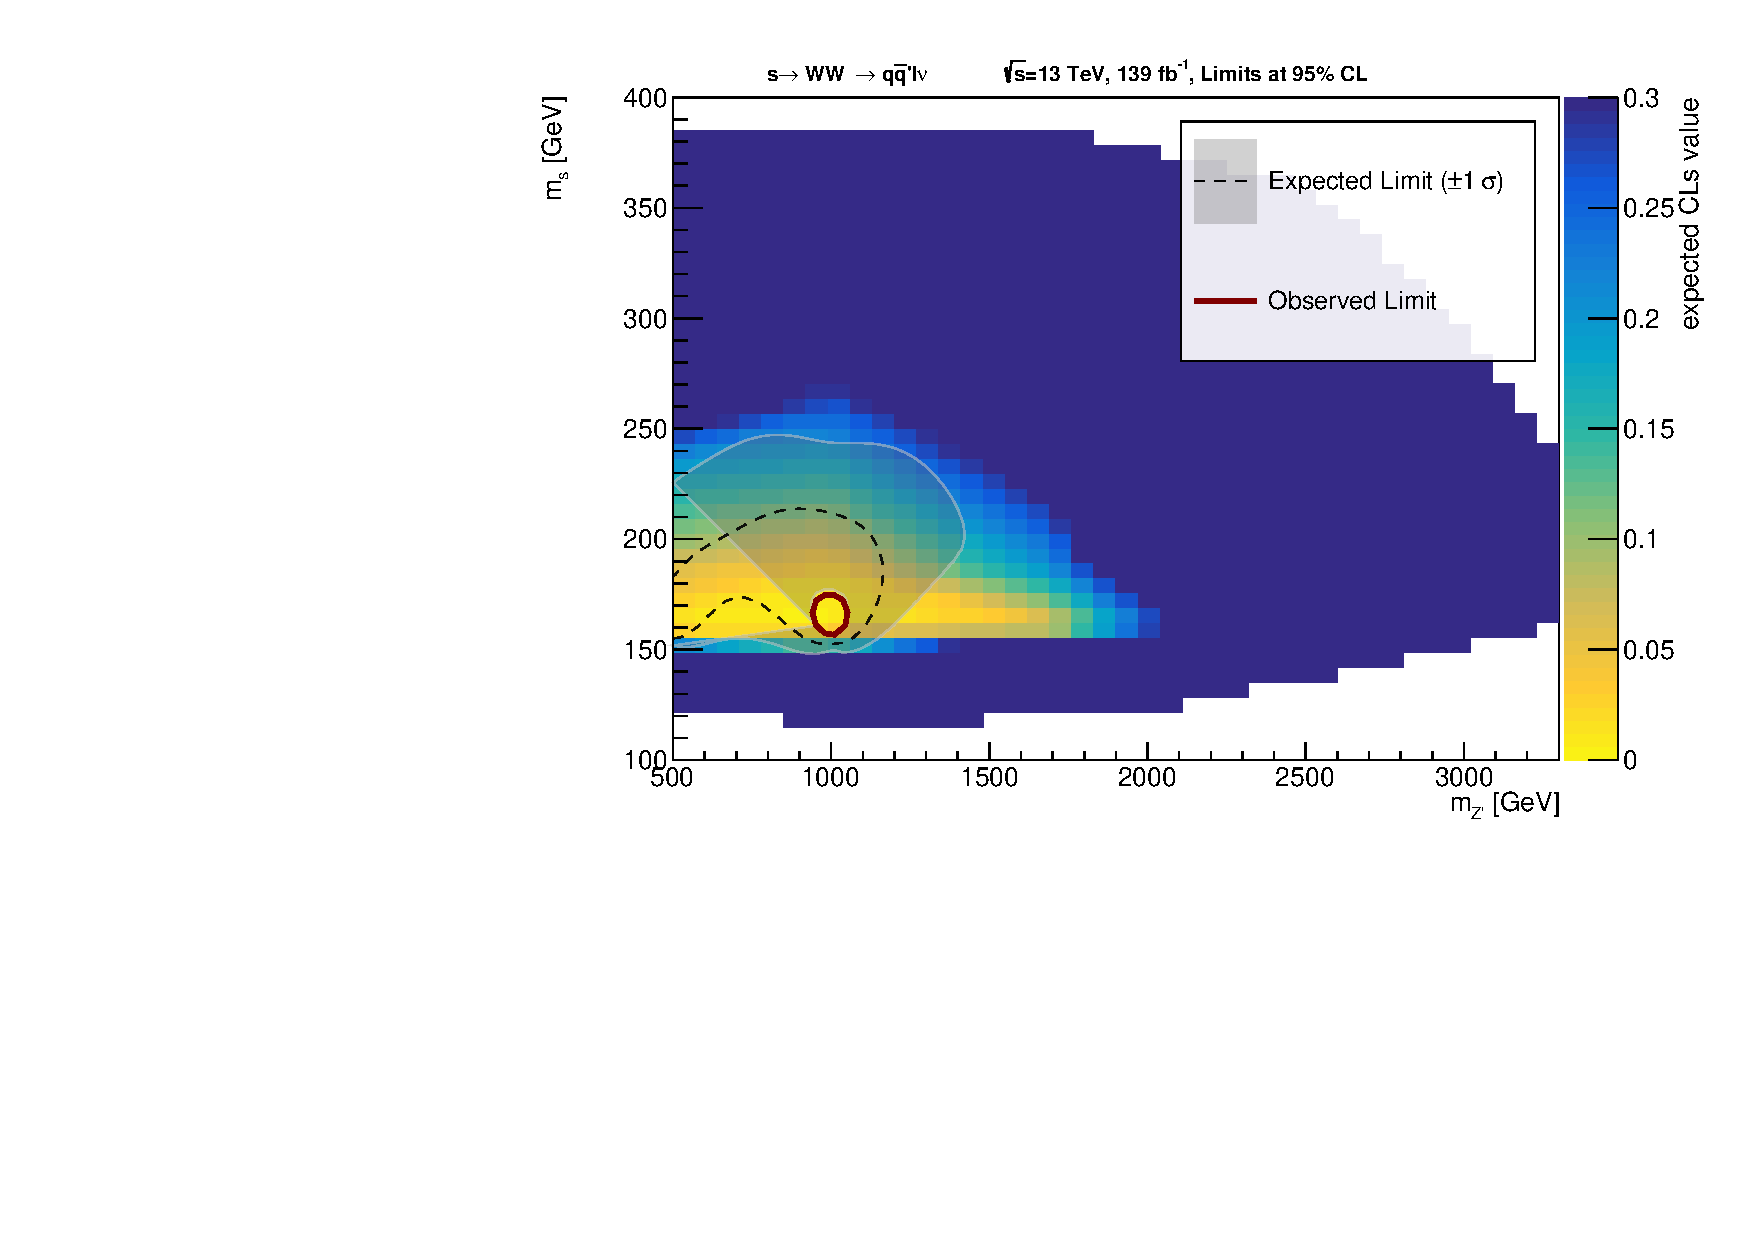
\includegraphics[width=\textwidth]{Figures/8/unblinded_0_15_nosig.pdf}
    \caption{\(g_q=0.15\)}\label{fig:unblinded_0.15}
  \end{subfigure} \vspace{1em}
  \caption[]{Range of \ms and \mZp in the DH signal model excluded by the search for various choices of the signal strength \(mu\) which coherently scales the production rate of the signal model at all \ms and \mZp.}
  \label{fig:limits_vary_mu_sig}
\end{figure}